%%% PREAMBLE - Do not touch %%%%%%%%%%%%%%%%%%%%%%%%%%%%%%%%%%%%%%%%%%%%%%%%%%%%%%
\documentclass[10pt,twocolumn,letterpaper]{article}
\usepackage[utf8]{inputenc}
\usepackage[portuges,brazil,english]{babel}
\usepackage{model}
\usepackage{times}
\usepackage{epsfig}
\usepackage{graphicx}
\usepackage{amsmath}
\usepackage{amssymb}
\usepackage{color}
\usepackage[pagebackref=true,breaklinks=true,letterpaper=true,colorlinks,bookmarks=false]{hyperref}

\cvprfinalcopy % *** Uncomment this line for the final submission
\def\httilde{\mbox{\tt\raisebox{-.5ex}{\symbol{126}}}}
\ifcvprfinal\pagestyle{empty}\fi

\newcommand{\TODO}[1]{TODO: #1}
\newcommand{\CITEONE}[2]{\mbox{#1 \cite{#2}}}
\newcommand{\CITETWO}[3]{\mbox{#1 and #2 \cite{#3}}}
\newcommand{\CITEN}[2]{\mbox{#1 et al. \cite{#2}}}

%%% Paper beginning %%%%%%%%%%%%%%%%%%%%%%%%%%%%%%%%%%%%%%%%%%%%%%%%%%%%%%%%%%%%%%
\begin{document}

%%% Title and authors %%%%%%%%%%%%%%%%%%%%%%%%%%%%%%%%%%%%%%%%%%%%%%%%%%%%%%%%%%%%
\title{MC886 - Trabalho prático 2}
\author{Guilherme P. Gonçalves (RA 091429)}

%%% Abstract %%%%%%%%%%%%%%%%%%%%%%%%%%%%%%%%%%%%%%%%%%%%%%%%%%%%%%%%%%%%%%%%%%%%%
\maketitle
\begin{abstract}
Este trabalho explorou técnicas de redução de dimensionalidade no contexto de uma aplicação de reconhecimento de faces. Diversas variações de um algoritmo de reconhecimento de faces utilizando Principal Component Analysis e Linear Discriminant Analysis foram implementadas e testadas sobre um conjunto de aproximadamente 3 mil fotografias de pessoas.
\end{abstract}

%%% Introduction %%%%%%%%%%%%%%%%%%%%%%%%%%%%%%%%%%%%%%%%%%%%%%%%%%%%%%%%%%%%%%%%%
\section{Introdução}

Algoritmos de redução de dimensionalidade são fundamentais em diversas aplicações de aprendizado de máquina na medida em que podem reduzir drasticamente a complexidade de um modelo e torná-lo muito mais eficiente em termos computacionais.

Neste trabalho, foram exploradas as aplicações de duas técnicas de redução de dimensionalidade, Principal Component Analysis (PCA) e Linear Discriminant Analysis (LDA), a um problema de reconhecimento de faces em que os dados de treinamento e teste eram imagens de pessoas cujos pixels deveriam ser utilizados como \emph{feature vectors}.

A Seção \ref{sec-problem} descreve em mais detalhes a proposta deste trabalho, enquanto a Seção \ref{sec-algorithm} descreve algumas particularidades dos algoritmos desenvolvidos e de suas implementações. A Seção \ref{sec-experiments} contém os resultados experimentais da aplicação dos algoritmos a um conjunto de imagens de faces.

\section{O problema analisado}
\label{sec-problem}

O problema analisado neste estudo é uma aplicação clássica da área de aprendizado de máquina: o reconhecimento de faces. Especificamente, dado um conjunto de 3414 fotografias de pessoas em tons de cinza, dividido em um grupo de "referência" de 3214 imagens e outro de "consulta" contendo 200 imagens, construiu-se de diversas formas um banco de dados de referência (BDR) a partir do primeiro grupo e um banco de dados de consulta (BDC) a partir do segundo. Avaliou-se então o efeito das diferentes formas de construir tais bancos de dados sobre o número de classificações corretas das imagens em BDC usando BDR no aprendizado.

Como restrição prévia, todas as imagens deveriam ser associadas a \emph{feature vectors} dados pelos valores de seus pixels linearizados em ordem de linhas. Ou seja, para uma imagem de 50x50 pixels, o \emph{feature vector} deveria ter dimensão 2500, sendo que as primeiras 50 dimensões são os valores dos pixels na primeira linha da matriz da imagem. O uso de \emph{feature vectors} grandes sugere a aplicação de técnicas de redução de dimensionalidade, que foram o grande objeto de exploração deste trabalho.

\section{Descrição dos algoritmos}
\label{sec-algorithm}

Todos os algoritmos implementados para este trabalho eram variantes de um método geral, que consiste em computar os \emph{feature vectors} a partir das imagens e, para cada imagem em BDC, encontrar a imagem mais próxima a ela no BDR e usá-la como classificação. Sobre essa ideia geral foram variados os métodos de construção de \emph{feature vectors} e de cálculo de distância entre eles.

Uma mesma etapa de pré-processamento das imagens precedeu a aplicação de todos os algoritmos, visando a tornar as imagens mais representativas das pessoas retratadas. Para cada uma das imagens conheciam-se as posições dos centros dos dois olhos, do nariz e da boca. A etapa de pré-processamento usava essas informações para produzir uma imagem de tamnho reduzido (o mesmo tamanho para todas as imagens) e que tentasse capturar a maior parte da face representada.

A técnica de recorte do rosto utiliza proporções simples comumente aplicadas por ilustradores ao desenhar rostos humanos \cite{FacialProportions:2010:Online}. Por exemplo, a distância entre os cantos internos dos olhos é aproximadamente igual à largura de um olho, e a largura da face é próxima de cinco vezes essa largura. Uma vez recortado o rosto, a imagem é redimensionada para um tamanho comum. A Figura \ref{fig-cropping} apresenta uma imagem original (reduzida para ilustração apenas) à esquerda, e sua versão pré-processada em tamanho 50x50 à direita. Na seção \ref{sec-experiments} foram testados diferentes tamanhos de imagens pré-processadas.

\begin{figure}
\begin{center}
	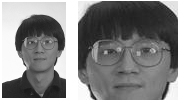
\includegraphics[width=0.99\columnwidth]{pics/cropping.png}
	\caption{Imagem original (esq.) e pré-processada (dir.), após o recorte da face e redimensionamento para 50x50.}
	\label{fig-cropping}   
\end{center} 
\end{figure}  

Os algoritmos testados operam a seguir sobre essas imagens pré-processadas. Esses algoritmos são denominados \emph{plain}, \emph{pca}, \emph{lda}, \emph{pca.lda} e \emph{lda.pca}.

O algoritmo \emph{plain}, considera como \emph{feature vectors} as imagens inteiras, com cada dimensão dada pelo valor do pixel correspondente (normalizado pelo valor máximo de 255, ou seja, variando no intervalo de 0 a 1).

Os algoritmos \emph{pca} e \emph{lda} usam PCA e LDA sobre os \emph{feature vectors} do algoritmo \emph{plain}. Especificamente, as técnicas de redução de dimensionalidade são aplicadas aos vetores em BDR para encontrar uma transformação com dimensionalidade reduzida; essa transformação era depois aplicada ao BDC antes das consultas. Para o algoritmo LDA, foi utilizada como classe a pessoa retratada na foto. Os algoritmos \emph{pca.lda} e \emph{lda.pca} usam PCA sobre os resultados do LDA e LDA sobre os resultados do PCA, respectivamente.

Uma vez calculados os  \emph{feature vectors} para cada imagem do BDR e BDC, as imagens do BDC são classificadas utilizando a imagem com vetor mais próximo no BDR, dado, para todos os algoritmos acima, pela distância Euclidiana. Também foram conduzidos, na seção \ref{sec-experiments}, experimentos usando norma L-1.

O algoritmo PCA pode ser configurado para escolher quanta "energia" dos vetores originais será capturada pelos vetores de dimensionalidade reduzida. Foram conduzidos experimentos utilizando 95% e 99% para essa variável.

Cabe, finalmente, notar alguns aspectos da implementação dos algoritmos, feita inteiramente em R.

Para atingir maior eficiência, a cada consulta a busca pelo vetor mais próximo no BDR foi feita utilizando uma estrutura de dados k-d tree encontrada no pacote FNN.

A linguagem R contém duas funções, princomp e prcomp, para executar o cálculo da PCA. A primeira utiliza autovetores e autovalores para decompor a matriz de covariâncias, enquanto a segunda usa SVD. A primeira, embora muito mais rápida, está mais suscetível a erros numéricos e só funciona quando o número de vetores de entrada é maior que o número de dimensões. Como não se observaram diferenças nos resultados finais dos testes ao se utilizar as diferentes funções, as implementações dos algoritmos buscam usar princomp quando possível por razões de eficiência, recorrendo a prcomp em testes de grande dimensionalidade.


\section{Resultados experimentais}
\label{sec-experiments}

Esta seção contém os resultados experimentais da aplicação do algoritmo para um corpo de 18828 emails.

Para esses emails, construíram-se os feature vectors como na Seção \ref{sec-algorithm}. Foram utilizadas 1432 palavras como features, de forma que essa era a dimensão de cada feature vector. A título de ilustração, a Tabela \ref{tbl-feature-words} contém cinco feature words e os respectivos valores de idf.

\begin{table}
\begin{center}
\begin{tabular}{l*{6}{c}r}
Palavra & idf  \\
\hline
muslim & 3.9908979 \\
iron & 4.5960763 \\
specif & 3.0896625 \\
stuff & 2.9834855 \\
environm & 3.9794692 \\
\end{tabular}
\end{center}
\caption{Feature words e seus valores idf}
\label{tbl-feature-words}
\end{table}

A seguir, buscou-se um valor razoável de $k$ para o algoritmo k-means através do método do cotovelo. Nesse método, o faz-se k-means para diversos valores diferentes de $k$ e analisa-se um gráfico da distorção resultante, dada pela soma das distâncias de cada ponto ao centróide de seu respectivo cluster, para encontrar um valor $k^{*}$ em que a curva deixa de decrescer rapidamente, ou seja, a partir do qual adicionar clusters não descreve significativamente melhor os dados disponíveis. O valor $k^{*}$ assim encontrado é o valor mais adequado.

A fim de preservar recursos computacionais, e porque como parte da descrição problema sabia-se que o valor máximo de $k$ seria 100, fez-se a princípio uma busca grosseira para valores de $k$ variando de 2 a 100 de 5 em 5. A Figura \ref{fig-five-by-five} contém a curva de distorção para esse processo.

 

Uma abordagem parecida foi tentada utilizando como features palavras que apareciam em no mínimo $0.1\%$ em vez de $1\%$ dos textos. No entanto, o número adicional de features (nesse caso, 7473 palavras foram utilizadas) não trouxe diferença significativa no formato da curva, e apenas tornou o processamento proibitivamente mais caro no hardware disponível.

Embora não se observe na Figura \ref{fig-five-by-five} um "cotovelo" evidente, ela indica que a região inicial, para valores de $k$ abaixo de 50, deverá conter $k^{*}$. Para averiguar isso, fez-se a seguir um gráfico similar, desta vez para $k$ de 5 a 60, de 1 em 1. Esse gráfico pode ser visto na Figura \ref{fig-one-by-one}.

Novamente não se observa um "cotovelo" claro, mas da observação das Figuras \ref{fig-five-by-five} e \ref{fig-one-by-one} pode-se sugerir um valor de $k^{*} = 20$. O algoritmo k-means embutido na linguagem R foi então executado com um máximo de 100 iterações e 20 tentativas para os feature vectors e o valor escolhido de $k^{*}$. A Tabela \ref{tbl-centroids} mostra os centróides dos clusters obtidos dessa forma.

\begin{table}
\begin{center}
\begin{tabular}{l*{6}{c}r}
Cluster & Centróide \\
\hline
1 & eb2f9133b4b0bec6e81e1ed3fd6871ad.txt \\
2 & f21cc70562a389a74e140c1e40056297.txt  \\
3 & 29b01f5319a9856c1c4f09723773ec27.txt  \\
4 & af959473240dca5eccdb05302d0b8729.txt \\
5 & a9b0af073d3bb8077e12dc425b19a16d.txt \\
6 & 21c5def39d47ed609131635445d713f6.txt \\
7 & da29032bb3599fdfae59efaabeb0e00c.txt  \\
8 & 876a160d1de6899cf5a42f0ad14280ec.txt  \\
9 & d1612488548207a3a47843aa4b11946e.txt  \\
10 & 568dbca15836174d86fa49d6ae15759b.txt  \\
11 & 7c359f7b276c69a09f39de853613d661.txt  \\
12 & 00a8bead7c4c98afe18ce0dbbb1763a1.txt  \\
13 & 51fea6f8b25d31b044bc478f237ab2bc.txt  \\
14 & f1ecb5dcbc2c870130eb033074e5653e.txt \\
15 & 828542de06991d1aa4c175a574fde230.txt  \\
16 & 18b58765c5788629460ca2be1f5ae197.txt  \\
17 & 6c59d51c480725d6fc8b6efebcf6bbeb.txt   \\
18 & b958662c7fbe5a311db5a243a1bda205.txt  \\
19 & aa289fb4e31543bd4603c3ba8b181f6f.txt  \\
20 & 3ca6289ad6e0830ad81c57f0d0e573a0.txt  \\
\end{tabular}
\end{center}
\caption{Centróides para cada um dos clusters.}
\label{tbl-centroids}
\end{table}

O restante desta seção consiste em uma breve análise dos clusters obtidos, utilizando tanto o centróide quanto os três emails mais próximos dele.

A Tabela \ref{tbl-closest} contém os três emails mais próximos do centróide indicado na Tabela \ref{tbl-centroids} para cada um dos clusters.

\begin{table*}
\begin{center}
\begin{tabular}{ | l | l || l | l | p{8cm} |}
\hline
Cluster & Emails mais próximos & Cluster & Emails mais próximos \\
\hline
1 & \parbox[c][1.5cm]{6cm}{5b9632c4c3c57519facb45f2a5dd5a96.txt 71868b35bb0b811f7f5663f79a8c28ad.txt 0ee154d3e67ef3491d08c517bb6fe4df.txt} & 11 & \parbox[c][1.5cm]{6cm}{2755cab2f3e51f89ca0626c0a9abd270.txt 4c5e172dd2027a260ff57c97d445e0c8.txt d3defe1ce80c3e8e5f3690ff2de4bfd6.txt} \\
2 & \parbox[c][1.5cm]{6cm}{b2dc92abc4b68e5cdeb35387f8ed5f9d.txt 462269622ff446945d15b6d30654980c.txt 5a50f1acdd629680d3674615b9a338f7.txt} & 12 & \parbox[c][1.5cm]{6cm}{96b1a8d440f324d8f940eda1ad708688.txt 7a0b3d49a55a124dcc75c403420c0481.txt c522abec15bb519308450f94dfb40e3c.txt} \\
3 & \parbox[c][1.5cm]{6cm}{46d8a2cf039a2edd9fb76d8fe5b57a27.txt 2f95838d2fda44a43407c9e243e3384e.txt 72c8a757df1156692e96c7332737afd3.txt} & 13 & \parbox[c][1.5cm]{6cm}{36008db69e04ec4d33ede317ebc610e0.txt cc4d9d84fe5cf6c35ec8494274327f02.txt 2aabe5207a8473b97bd50e40f9edc05f.txt} \\
4 & \parbox[c][1.5cm]{6cm}{51f0c24f17369733f168eaeceac9ad8f.txt 2a14c92aad620ef59b6d0b87780f4814.txt decf2f483ed9c57954344fd6907ce901.txt} & 14 & \parbox[c][1.5cm]{6cm}{bdb3bc8a274e14e4502f451ecca48e1c.txt 5a84b4fdad31b7e2126f2e2666ec489d.txt cc3bf528d548f68f9a24035e52250c07.txt} \\
5 & \parbox[c][1.5cm]{6cm}{c0b40f790c6fce852050a1cd583b402e.txt 9268ca2ca808dfb3203493624d8de16d.txt c6d971c9a8a7e657850b2c02efe24b00.txt} & 15 & \parbox[c][1.5cm]{6cm}{aa9b5da52193ae6702e6bdb2b58c9689.txt d319f109965da97c9019c42eef7311e2.txt 6cd6904b27ee4c3fe30ca2f4ec328459.txt} \\
6 & \parbox[c][1.5cm]{6cm}{3ceb2061ab2d2c18bce8154a12992048.txt afa06f71e93f04f4a18e9093383b9dfe.txt 9eb334f10e9cc1ea237495af4b16179c.txt} & 16 & \parbox[c][1.5cm]{6cm}{c2237bdfcf99479a38c163d702129084.txt d3da10cf0cf00c4804340ff875a65ed4.txt 7f90830cc72af813b860f3507612d555.txt} \\
7 & \parbox[c][1.5cm]{6cm}{2adb9b7e74f340a7286f48ffee27c765.txt fcf4795a3ff768082c48123d3099228c.txt 9068f47025e17a92798bd6d501963f61.txt} & 17 & \parbox[c][1.5cm]{6cm}{063c99c35807c214821baf2322cd2a1f.txt c30b87a3cab64107d7645c7a3267a48e.txt 0ac219066196e61a5d6310599c39cb0b.txt} \\
8 & \parbox[c][1.5cm]{6cm}{933be2ef334f634b21ab972bbb3c7d5d.txt 6a60803a3f25cbf7afa977b0633fa784.txt 85686c1b3fcab0e81b51da08bbd80301.txt} & 18 & \parbox[c][1.5cm]{6cm}{78ee1bcf9ad28f01869e12cb8356b442.txt c2523343949c58ec7872a44890df9e90.txt 78787171952df493ac6df45743deb2a4.txt} \\
9 & \parbox[c][1.5cm]{6cm}{d14ca6250c73453f03f953fd4a932f91.txt 64bde302248786f3086758bad6eeed34.txt 437de825b1fc16f7214fb084d2bb8562.txt} & 19 & \parbox[c][1.5cm]{6cm}{3e9ddd1e7e87bac92ba60141d272112c.txt 44d6f3b22396ae4c3e38ba7c62bf76f3.txt 4719c3d122e0c7f65b672d8d62f92577.txt} \\
10 & \parbox[c][1.5cm]{6cm}{7beea049940fb8b12f43c48600abe1ec.txt 886483fadc2a405a5df48e7347bb037d.txt a8a044035ceee093af05f0c624fabdde.txt} & 20 & \parbox[c][1.5cm]{6cm}{61f339f0277cb05c595443666f7059e0.txt 341c946015fac9b47e9424e3b2d2cdd9.txt 3e4b63cf30a6c7c3b647f5f19274f62c.txt}  \\
\hline
\end{tabular}
\end{center}
\caption{Emails mais próximos do centróide para cada um dos clusters.}
\label{tbl-closest}
\end{table*}

Para o cluster 1, todos os emails destacados falam sobre porte de armas e conflitos civis. Pode-se inferir que o cluster 1 se refere à discussão sobre porte de armas por civis. Dos emails do cluster 2, o centróide e dois dos emails mais próximos envolvem astronomia, mas o terceiro, presumivelmente classificado erroneamente, fala sobre privacidade na Internet.

Todos os emails selecionados do cluster 3 discorrem sobre hockey -- especificamente, sobre o ex-jogador e comentarista Don Cherry. Os emails do cluster 4 também todos abordam o mesmo tema, a religião cristã e discussões sobre a Bíblia.

Dos emails no cluster 5, 3 (incluindo o centróide) mencionam formatos de arquivos de imagens digitais, e o restante fala sobre formatos de arquivos em Mac. Presume-se assim que o tema desse cluster seja processamento de imagens. No cluster 6, todos os emails falam sobre implementação de interfaces gráficas, mencionando conceitos como gerenciadores de janelas.

Dentre os emails no cluster 7, dois, incluindo o centróide, falam sobre placas de vídeo, e os demais falam sobre outras placas de hardware -- a palavra "card" parece ser determinante aqui. Os emails do cluster 8 discorrem sobre compra de carros.

Dentre os emails do cluster 9, o centroide e dois dos mais próximos a ele versam sobre motocicletas, e o restante sobre "waterski bikes", um veículo marinho similar a uma motocicleta. No cluster 10 foram agrupados emails sem corpo, com apenas assunto ou mesmo sem assunto.

Os emails do cluster 11 discutem conflitos étnicos e nazismo, enquanto os do cluster 12, embora abordem temas de tecnologia, não concordam em um tópico específico -- há emails sobre programação no sistema de janelas X, processos Unix, Windows 3.1 e programação em baixo nível.

Dos emails no cluster 13, três falam sobre hockey e um sobre baseball. Presumivelmente este cluster seria agregado ao cluster 3 em um experimento com $k$ menor.  Os emails do cluster 14 também abordam assuntos dispersos, como culinária, carros e processamento de imagens.

Os emails do cluster 15 falam sobre problemas de hardware em laptops, e os do cluster 16 discorrem sobre o conflito entre israelenses e palestinos. Os emails do cluster 17 discutem criptografia, e os do cluster 18 contém anúncios de vendas diversas.

Todos os emails do cluster 19 tratam de processamento de imagens, em uma possível concordância com o cluster 5. Finalmente, os emails do cluster 20 consistem em pessoas pedindo ou discutindo números de telefone.

Embora tenha-se observado alguma similaridade entre alguns pares de clusters, observa-se que o algoritmo proposto obteve resultados satisfatórios, em geral com todos os emails amostrados em cada cluster abordando os mesmos temas.

\section{Aspectos de implementação}
\label{sec-impl}

Além de explorar conceitos de classificação de textos, este trabalho também exercitou aspectos básicos de programação em R. Certas características da linguagem e restrições nos recursos computacionais disponíveis foram os principais fatores em algumas das decisões de implementação; essas decisões são discutidas nessa seção.

Um importante desafio encontrado no início do desenvolvimento deste projeto foram limitações da memória disponível no computador utilizado. Essa limitação se mostrou particularmente presente ao construir feature vectors grandes (versões iniciais do algoritmo usavam todo o dicionário $D$ como feature words), e foi mitigada tanto através de de uma seleção mais criteriosa das features quanto, principalmente, do uso de matrizes esparsas fornecidas pelo pacote "Matrix" em R, após a observação de que os feature vectors construídos eram sempre bastante esparsos.

Pelo que se observou desde o começo do desenvolvimento, a linguagem R fornece diferentes formas de se expressar uma mesma operação, e o tempo usado por cada uma delas pode variar em até uma ordem de magnitude. Por isso, parte significativa do tempo de desenvolvimento deste trabalho foi dedicado a encontrar áreas com problemas de performance usando a ferramenta de \emph{profiling} Rprof e otimizá-las.

Por exemplo, em loops que preenchem valores em um vetor (como o que computa o vetor $idf$), observou-se uma significativa melhora de performance ao utilizar vetores pré-alocados de tamanho fixo em vez de criar um vetor de tamanho pequeno e fazê-lo crescer a cada iteração. Por isso, a versão final do algoritmo faz múltiplas passadas sobre os emails de entrada, de forma a calcular de antemão os tamanhos dos vetores necessários. Por exemplo, o cálculo do número de emails contendo cada palavra é feito em uma passada posterior à que quebra os emails em palavras, para que se possa saber de antemão o tamanho do conjunto $D$.

Evita-se através da técnica de \emph{memoização} repetir a operação de quebra de emails em palavras, que seria necessária por todas as passadas: após a primeira vez que isso é feito, os resultados são salvos em memória e reutilizados. Felizmente, embora a memória disponível do sistema não seja suficiente para guardar os textos completos de todos os emails, ela foi capaz de guardar as palavras encontradas com facilidade.

Outra otimização útil foi a utilização das funções "Map" e "sapply" em lugar de construções explícitas de loop "for". Essa manipulação ainda abre espaço para fácil paralelização do código, que foi experimentada de forma superficial no final do projeto, tornando muito mais rápida a execução dos múltiplos k-means usados no método do cotovelo.

Como resultado dessas otimizações, é possível rodar o projeto completo usando o valor $k = 20$ e obter os resultados da Seção \ref{sec-experiments} em aproximadamente uma hora e meia na máquina de testes, um MacBook Pro com 16GB de memória com processador quad-core Core i7. Outras otimizações possíveis, mas não implementadas, seriam uma implementação específica do algoritmo k-means (em vez de utilizar aquele provido pelo ambiente R), e uso mais extensivo de paralelismo.

\section{Conclusão e melhorias futuras}
Este trabalho explorou de forma bem sucedida técnicas simples de classificação de texto e conceitos básicos de programação em R. A presença de clusters com assuntos similares (e outros sem nenhum assunto identificável) indica que uma melhoria futura poderia ser refinar a escolha de $k$, embora de forma geral os resultados tenham sido satisfatórios. Além disso, futura otimização da implementação, em particular de seu consumo de memória, pode tornar factível explorar o uso de feature vectors maiores ou mais iterações do algoritmo k-means, potencialmente produzindo resultados melhores.

%%% References %%%%%%%%%%%%%%%%%%%%%%%%%%%%%%%%%%%%%%%%%%%%%%%%%%%%%%%%%%%%%%%%%%%
{\small
\bibliographystyle{unsrt}
\bibliography{references}
}

\end{document}
